\documentclass[12pt, a4paper, titlepage]{article}

\usepackage[a4paper, includeheadfoot, margin=2.54cm]{geometry}
\usepackage{graphicx}
\usepackage[dvipsnames]{xcolor}
\usepackage{sectsty}
\usepackage{titling}
\usepackage{fancyhdr}
\usepackage{pgfplots}
\usepackage{tikz}
\usepackage{tikz-3dplot}
\usetikzlibrary{arrows.meta}
\usetikzlibrary{shapes.geometric, arrows}
\usepackage{mathtools}
%\usepackage[ngerman]{babel}
\usepackage[utf8]{inputenc}
\usepackage{paralist}
\usepackage{color}
\usepackage{eso-pic}
\usepackage{wrapfig}
\usepackage{amssymb}
\usepackage{chemfig}
\usepackage{multirow}
\usepackage{array}
\usepackage{multicol}
\usepackage{calc}
\usepackage{ragged2e}
\usepackage{mathtools}
\usepackage{empheq}
\usepackage{colortbl}
\usepackage{pifont}
\usepackage{savesym}
\usepackage[font=small]{caption}
\usepackage{marvosym}
\usepackage{braket}
\usepackage{anyfontsize}
\usepackage{listings}
\usepackage{makecell}
\usepackage{svg}
\usepackage{mdframed}
\usepackage{extarrows}
\PassOptionsToPackage{obeyspaces}{url}
\usepackage[pdftex, pdfauthor={Philipp A. Huber}, pdftitle={The Bible of Physics}, colorlinks,
pdfpagelabels,
pdfstartview = FitH,
bookmarksopen = true,
bookmarksnumbered = true,
linkcolor = black,
plainpages = false,
hypertexnames = false,
citecolor = black, urlcolor=black] {hyperref}


%Dokumenteinstellungen
\definecolor{myblue}{RGB}{212,217,255}
\definecolor{myblue2}{RGB}{40,40,115}
\definecolor{myblack}{RGB}{14,14,14}
\definecolor{mygrey}{RGB}{240,240,240}
\pagestyle{fancy}
\lhead{HPC}
\rhead{Unix Commands}
\chead{Philipp Huber (14-936-694)}
\cfoot{\thepage}
\setcounter{secnumdepth}{0}
\tikzstyle{block} = [rectangle, minimum width = 4cm, minimum height = 1cm, fill = myblue, text centered]
\tikzstyle{gblock} = [rectangle, minimum width = 4cm, minimum height = 1cm, fill = mygrey, text centered]
\tikzstyle{arrow} = [thick,->,>=stealth]
\tikzstyle{tarrow} = [very thick,->,>=stealth]
\tikzstyle{uarrow} = [ultra thick,->,>=stealth]
\setlength\parindent{0pt}
\lstset{basicstyle=\ttfamily\small,breaklines=true}
%\partfont{\color{myblue2}} 
%\sectionfont{\color{myblue2}} 
%\subsectionfont{\color{myblue2}}


%New Commands
\newcommand{\bx}[1]{
    \begin{center}
  	    \fboxrule2mm
	    \fcolorbox{myblue}{myblue}{
	    \begin{math}
	    #1
        \end{math}
        }
    \end{center}
}

\newcommand{\bbx}[1]{
	    \begin{mdframed}[backgroundcolor=myblue, innertopmargin=10pt, innerbottommargin=10pt, topline=false, bottomline=false, rightline=false, leftline=false]
	    #1
    \end{mdframed}
}

\newcommand{\gbx}[1]{
	    \begin{mdframed}[backgroundcolor=mygrey, innertopmargin=10pt, innerbottommargin=10pt, topline=false, bottomline=false, rightline=false, leftline=false]
	    #1
    \end{mdframed}
}        


\newcommand{\wbx}[1]{
    \begin{center}
        \fboxrule2mm
	    \fcolorbox{white}{white}{
	    \begin{math}
	    #1
        \end{math}
        }
    \end{center}
}
\newcommand{\myref}[2]{\hyperref[#2]{\textcolor{myblue2}{\MVRightarrow} \hspace{-0.1cm}\textit{#1}} (Seite \pageref{#2})}
\newcommand{\tocref}[2]{\hyperref[#2]{\textcolor{myblue2}{\MVRightarrow} \hspace{-0.1cm}\textsc{#1}}}
\newcommand{\cd}{\cdot}
\renewcommand{\arraystretch}{1.5}
\newcommand{\abl}{\text{d}}
\newcounter{def}
\newcounter{bsp}
\newcounter{anl}
\newcommand{\defi}[1]{\textbf{Definition \stepcounter{def}\arabic{def}} \textbf{(#1)}}
\newcommand{\bsp}{\textbf{Beispiel \stepcounter{bsp}\arabic{bsp}} }
\newcommand{\anl}{\textbf{Anleitung \stepcounter{anl}\arabic{anl}} }
\newcommand{\R}{\mathbb{R}}
\newcommand{\C}{\mathbb{C}}
\newcommand{\N}{\mathbb{N}}
\newcounter{src}
\newcommand{\src}[1]{\stepcounter{src}\expandafter\xdef\csname#1\endcsname {\arabic{src}}\hyperref[Quellenverzeichnis]{[\arabic{src}]}}
\newcommand{\iql}[4]{#1$\quad$#2: \url{#3} (#4)}
\newcommand{\itm}{\item[\tiny\color{myblue2}\ding{110}]}
\newcommand{\formel}[1]{\vspace{0.3cm}
\begin{gather*}
	#1
\end{gather*}\par
\vspace{0.3cm}
\noindent}
%\expandafter\def\expandafter\UrlBreaks\expandafter{\UrlBreaks}%  save the current one
%  {\do\a\do\b\do\c\do\d\do\e\do\f\do\g\do\h\do\i\do\j%
%  \do\k\do\l\do\m\do\n\do\o\do\p\do\q\do\r\do\s\do\t%
%  \do\u\do\v\do\w\do\x\do\y\do\z\do\A\do\B\do\C\do\D%
%  \do\E\do\F\do\G\do\H\do\I\do\J\do\K\do\L\do\M\do\N%
%  \do\O\do\P\do\Q\do\R\do\S\do\T\do\U\do\V\do\W\do\X%
%  \do\Y\do\Z}
\newcommand{\bibspace}{\hspace*{0.83cm}}
\newcommand{\vp}{\vspace{1cm}}
\newcommand{\der}{\text{d}}

\tikzstyle{arrow} = [->]
\tikzset{
fermion/.style={thick,draw=black, postaction={decorate},
    decoration={markings,mark=at position 1 with {\arrow[black]{triangle 45}}}}}













%%%%%%%%%%%%%%%%%%%%%%%%%%%%%%%%%%%%%%%%%%%%%%%%%%%%%%%%%%%%%%%%%%%%%%%%%%%%%%%%%%%%%%%%%%%%%%%%%%%%%%%%%%%%%%%%%%%%%%%%%%%%%%%%%%%%%%%%%%%%%%%%%%%%%%%%%%%%%%%%%%%%%%%%%%%%%%%%%%%%%%%%%%%%%%%%%%%%%%%%%%%%%%%%%%%%%%%%%%%%%%%%%%%%%%%%%%%%%%%%%%%%%%%%%%%%%%%%%%%%%%%%









%Dokumentbeginn
\begin{document}

\lstset{language=Fortran}




%Titelseite
\begin{titlepage}
	\enlargethispage{1cm}
	\color{white}
	\vspace*{1cm}
	\tikz[remember picture, overlay] \node[opacity=0.9, below=0cm] at (current page.north)      {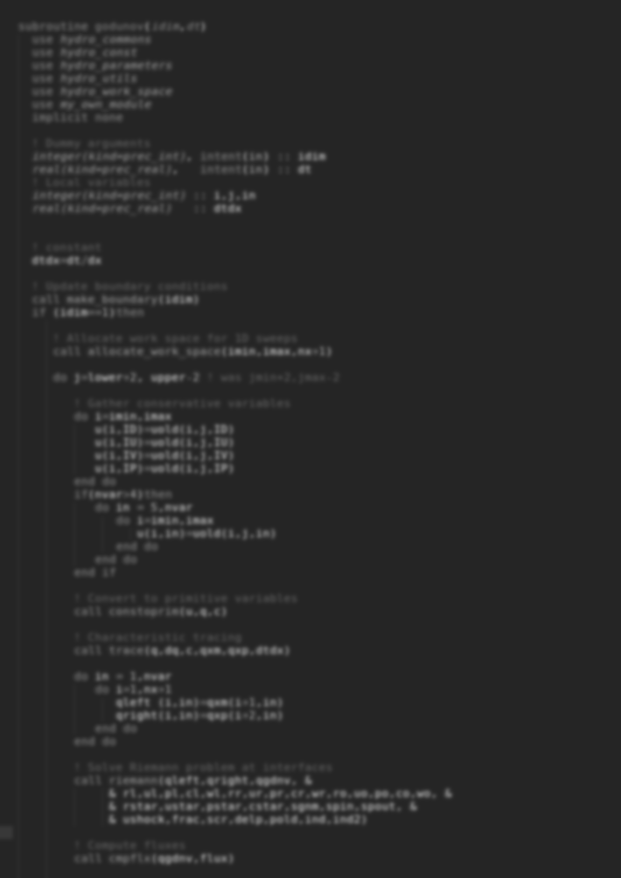
\includegraphics[width=21.40cm]{pictures/code2.png}};	
    \begin{tikzpicture}[remember picture, overlay]
    \node (A)  at (current page.south west) {};
    \node (B)  at (current page.north west) {};
    \node (C)  at (current page.north east) {};
    \node (D)  at (current page.south east) {};
    \coordinate (cA) at (A) ;
    \coordinate (cB) at (B);
    \coordinate (cC) at (C);
    \coordinate (cD) at (D) ;
    \draw[line width=6mm] (cA) -- (cB) -- (cC) -- (cD) -- cycle;
    \node[white, left] at (16, -3) {\sffamily \fontsize {33}{33} \selectfont Parallelizing The Hydro Code};
    \node[white, left] at (16, -5.15) {\sffamily \fontsize{23}{23}\selectfont Hannes Imboden, Philipp A. Huber};
    \node[white, left] at (16, -9) {\sffamily \fontsize{18}{18}\selectfont High Performance Computing};
    \node[white, left] at (16, -10) {\sffamily \fontsize{18}{18}\selectfont Final Project};
    \node[white, left] at (16, -11) {\sffamily \fontsize{18}{18}\selectfont June 2018};
    \end{tikzpicture}
\end{titlepage}


%\begin{titlepage}
%	\enlargethispage{1cm}
%	\color{white}
%	\vspace*{1cm}
%	\tikz[remember picture, overlay] \node[opacity=0.9, below=0cm] at (current page.north)      {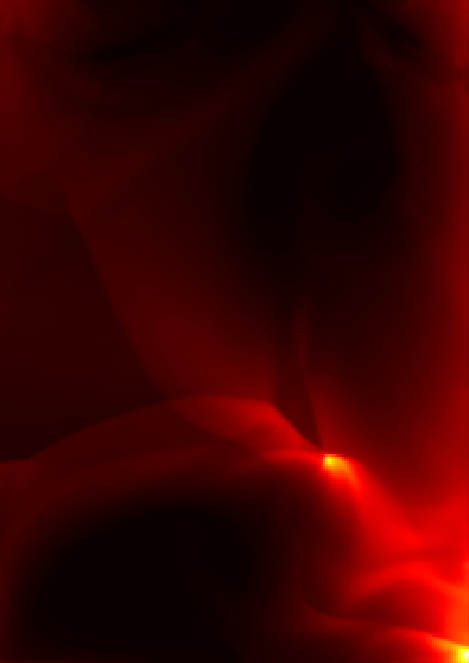
\includegraphics[width=21.40cm]{pictures/hydro2.png}};	
%    \begin{tikzpicture}[remember picture, overlay]
%    \node (A)  at (current page.south west) {};
%    \node (B)  at (current page.north west) {};
%    \node (C)  at (current page.north east) {};
%    \node (D)  at (current page.south east) {};
%    \coordinate (cA) at (A) ;
%    \coordinate (cB) at (B);
%    \coordinate (cC) at (C);
%    \coordinate (cD) at (D) ;
%    \draw[line width=6mm] (cA) -- (cB) -- (cC) -- (cD) -- cycle;
%    \node[white, right] at (-0.15, -3) {\sffamily \fontsize {33}{33} \selectfont Parallelizing the Hydro Code};
%    \node[white, right] at (0, -5) {\sffamily \fontsize{23}{23}\selectfont Hannes F. Imboden, Philipp A. Huber};
%    \node[white, right] at (0, -10) {\sffamily \fontsize{18}{18}\selectfont High Performance Computing};
%    \node[white, right] at (0, -11) {\sffamily \fontsize{18}{18}\selectfont Final Project};
%    \node[white, right] at (0, -12) {\sffamily \fontsize{18}{18}\selectfont June 2018};
%    \end{tikzpicture}
%\end{titlepage}


\newpage
%Contents
\clearpage
\thispagestyle{plain}
\pagenumbering{Roman}
\setcounter{page}{1}
{\pagestyle{plain}
\tableofcontents\label{toc}
\clearpage
\pagenumbering{arabic}
\setcounter{page}{1}
%\thispagestyle{plain}}
%\begingroup
%\let\clearpage\relax
%\listoffigures
%\endgroup
%\begingroup
%\let\clearpage\relax
%\listoftables
%\endgroup




\newpage
\section{Hydro Code Explained}

The hydro code is a simulation of a fluid or gas in an enclosed system. The initial conditions are set as to generate an unperturbed, homogeneous environment. Then, one can introduce points of higher or lower pressure or density to imitate an explosion or a jet. The code then calculates the propagation of this perturbation using Godunov's method and outputs each frame as a single file, which can be used to create an animation.\\
%The method used to calculate the dynamics of the fluid is the Godunov's.

There are five main components with different functionality to this Fortran based code:
\begin{itemize}
	\item \texttt{main.f90}
	\begin{itemize}
		\item calls \texttt{init\_hydro} to initialize the grid with the initial conditions
		\item executes the main time loop by calling
		\begin{itemize}
		\item \texttt{cmpdt} to compute the time step
		\item \texttt{godunov} to calculate the fluid dynamics
		\item \texttt{output} to generate output data
		\end{itemize}
	\end{itemize}
	\item \texttt{module\_hydro\_principal.f90} contains the subroutines
	\begin{itemize}
		\item \texttt{init\_hydro}
		\item \texttt{cmpdt}
		\item \texttt{godunov} which calls
		\begin{itemize}
				\item \texttt{make\_boundary} to set the upper, lower, left and right boundaries of the grid
				\item \texttt{allocate\_work\_space}/\texttt{deallocate\_work\_space} to (de)allocate space in the memory
				\item other subroutines for calculation purposes
			
		\end{itemize}
	\end{itemize}
	\item \texttt{module\_hydro\_utils.f90} contains
	\begin{itemize}
		\item \texttt{make\_boundary}
		\item other subroutines
	\end{itemize}
	\item \texttt{module\_hydro\_IO.f90} contains the subroutines
	\begin{itemize}
		\item \texttt{read\_params} to read the parameters from the \texttt{input.nml} file
		\item \texttt{output}
	\end{itemize}
	\item \texttt{module\_hydro\_commun.f90} contains 
	\begin{itemize}
		\item \texttt{allocate\_work\_space}/\texttt{deallocate\_work\_space}
		\item various other subroutines, mainly to define the variables used elsewhere in the code
	\end{itemize}		
\end{itemize}

Additionally, there are several input files to set the grid size with width $nx$ and height $ny$ and other initial conditions.








\section{Parallelization Techniques}
\subsection{MPI}

\subsubsection{Introduction}
MPI stands for \textit{message passing interface}. This refers to the fact that parallel computing occupies multiple CPUs to fasten up the execution of a code. As these CPUs work independently and with their own associated memory, they will have to communicate in some way; this is what MPI does.\\
The advantage of MPI over other libraries is that one has much more control over how the code is parallelized. The programmer can explicitly choose how the different cores communicate to each other and which information they share.\\
On the other hand, this freedom makes parallelizing a code a much more complex problem than it could be with other libraires. It requires quite a deep understanding of how the code works to know where and what to adjust.


\vp
\subsubsection{Parallelization Process}
%
%\begin{figure}[h!]
%	\begin{minipage}{0.7\linewidth}
The main idea was to split the initial grid horizontally into equally sized parts in assigning each core a certain portion of it. Each process would then calculate the evolution of the fluid in his portion only. Finally, these different parts would be merged together to recreate the grid with its original size. This \textcolor{red}{merging} is where the main part of the paralellization process is happening:\\
For a process to be able to calculate a given pixel of its grid, it needs information of its four neighbouring pixels. Thus, to calculate the values of the lower and upper most pixels within its grid part, they need access to the calculated values from the processes above and below. For this purpose, the so called \textit{ghost cells} were introduced. These are one-dimensional rows of pixels that only exist for calculation purposes, but are not present in the actual simulation.
%	\end{minipage}	
%	\hfill
%	\begin{minipage}{0.28\linewidth}
%		\resizebox{0.9\linewidth}{1.4\linewidth}{
%		\begin{tikzpicture}[>=triangle 60]
%			\draw (0, 2) -- (0, 0) -- (5, 0) -- (5, 2) node [right = -2.5cm, below = 0.2cm] {\LARGE process $N +1$};
%			\draw (0, 0) -- (5, 0) -- (5, -1) -- (0, -1) -- (0, 0) node [right = 2.5cm, below = 0.1cm] {\LARGE lower + 3};
%			\draw [line width = 2.5pt] (0, 0) -- (5, 0);
%			\draw (0, -1) -- (5, -1) -- (5, -2) -- (0, -2) -- (0, -1) node [right = 2.5cm, below = 0.1cm] {\LARGE lower + 2};
%			\draw (0, -2) -- (5, -2) -- (5, -3) -- (0, -3) -- (0, -2) node [right = 2.5cm, below = 0.1cm] {\LARGE lower + 1};
%			\draw (0, -3) -- (5, -3) -- (5, -4) -- (0, -4) -- (0, -3) node [right = 2.5cm, below = 0.1cm] {\LARGE lower};
%			
%			\draw (0, -6) -- (5, -6) -- (5, -7) -- (0, -7) -- (0, -6) node [right = 2.5cm, below = 0.1cm] {\LARGE upper};
%			\draw (0, -7) -- (5, -7) -- (5, -8) -- (0, -8) -- (0, -7) node [right = 2.5cm, below = 0.1cm] {\LARGE upper -1};
%			\draw (0, -8) -- (5, -8) -- (5, -9) -- (0, -9) -- (0, -8) node [right = 2.5cm, below = 0.1cm] {\LARGE upper -2};
%			\draw (0, -9) -- (5, -9) -- (5, -10) -- (0, -10) -- (0, -9) node [right = 2.5cm, below = 0.1cm] {\LARGE upper -3};
%			\draw (0, -12) -- (0, -9) -- (5, -9) -- (5, -12) node [right = -2.5cm, below = -1cm] {\LARGE process $N$};
%			\draw [line width = 2.5pt] (0, -10) -- (5, -10);
%			\draw [decorate,decoration={brace,amplitude=10pt,mirror,raise=4pt}, thick,yshift=0pt]
%(5.5,-2) -- (5.5,0) node [black,xshift=0.8cm] {};
%			\draw [decorate,decoration={brace,amplitude=10pt,mirror,raise=4pt}, thick,yshift=0pt]
%(5.5,-4) -- (5.5,-2) node [black,xshift=0.8cm] {};
%			\draw [decorate,decoration={brace,amplitude=10pt,mirror,raise=4pt},  thick,yshift=0pt]
%(5.5,-8) -- (5.5,-6) node [black,xshift=0.8cm] {};
%			\draw [decorate,decoration={brace,amplitude=10pt,mirror,raise=4pt}, thick,yshift=0pt]
%(5.5,-10) -- (5.5,-8) node [black,xshift=0.8cm] {};
%			\draw (6, -1) -- (7, -1) -- (7, -7);
%			\draw (6, -9) -- (8, -9) -- (8, -3);
%    		\draw [arrow] (7, -7) -- (6, -7);
%    		\draw [arrow] (8, -3) -- (6, -3);
%		\end{tikzpicture}
%		}
%		\caption{Communication}
%		\label{fig:tikz}
%		\end{minipage}
%\end{figure}

\begin{figure}[h!]
\begin{center}
		\begin{minipage}{0.35\linewidth}
		\resizebox{1.1\linewidth}{1.4\linewidth}{
		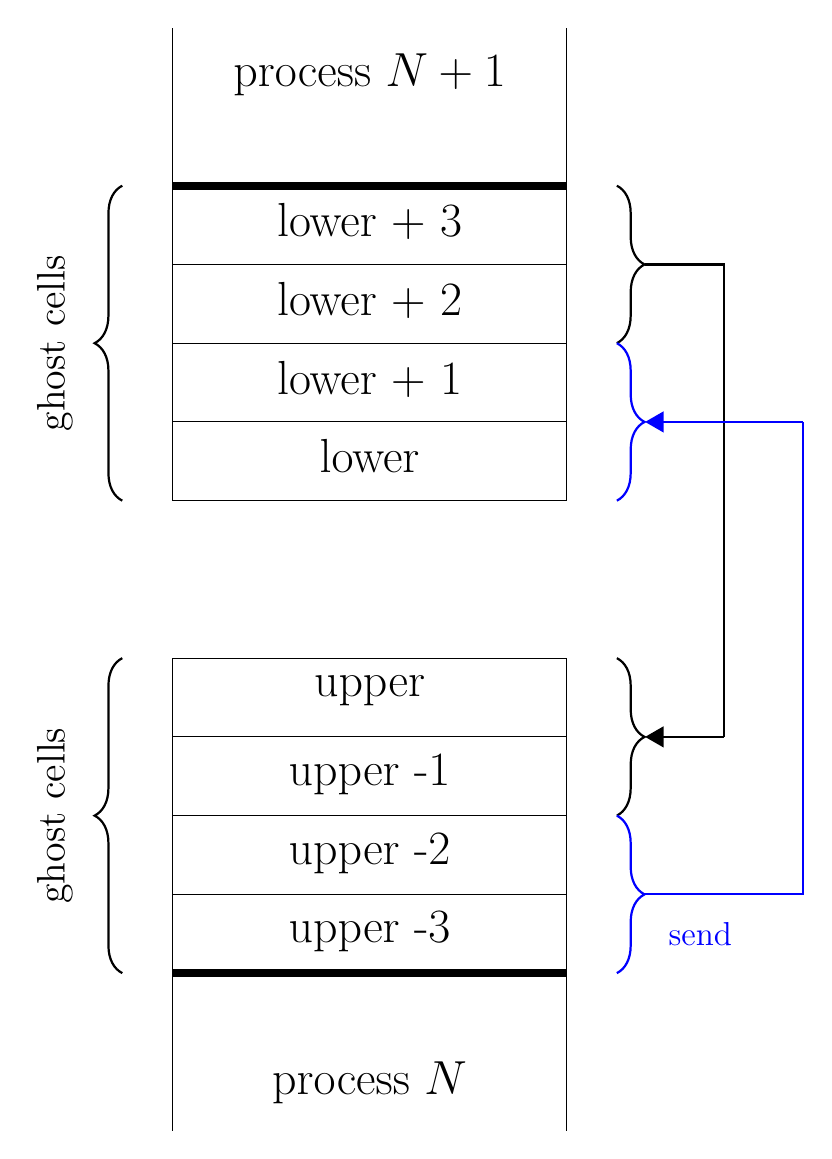
\begin{tikzpicture}[>=triangle 60]
			\draw (0, 2) -- (0, 0) -- (5, 0) -- (5, 2) node [right = -2.5cm, below = 0.2cm] {\LARGE process $N +1$};
			\draw (0, 0) -- (5, 0) -- (5, -1) -- (0, -1) -- (0, 0) node [right = 2.5cm, below = 0.1cm] {\LARGE lower + 3};
			\draw [line width = 3pt] (0, 0) -- (5, 0);
			\draw (0, -1) -- (5, -1) -- (5, -2) -- (0, -2) -- (0, -1) node [right = 2.5cm, below = 0.1cm] {\LARGE lower + 2};
			\draw (0, -2) -- (5, -2) -- (5, -3) -- (0, -3) -- (0, -2) node [right = 2.5cm, below = 0.1cm] {\LARGE lower + 1};
			\draw (0, -3) -- (5, -3) -- (5, -4) -- (0, -4) -- (0, -3) node [right = 2.5cm, below = 0.1cm] {\LARGE lower};
			
			\draw (0, -6) -- (5, -6) -- (5, -7) -- (0, -7) -- (0, -6) node [right = 2.5cm, below = 0.1cm] {\LARGE upper};
			\draw (0, -7) -- (5, -7) -- (5, -8) -- (0, -8) -- (0, -7) node [right = 2.5cm, below = 0.1cm] {\LARGE upper -1};
			\draw (0, -8) -- (5, -8) -- (5, -9) -- (0, -9) -- (0, -8) node [right = 2.5cm, below = 0.1cm] {\LARGE upper -2};
			\draw (0, -9) -- (5, -9) -- (5, -10) -- (0, -10) -- (0, -9) node [right = 2.5cm, below = 0.1cm] {\LARGE upper -3};
			\draw (0, -12) -- (0, -9) -- (5, -9) -- (5, -12) node [right = -2.5cm, below = -1cm] {\LARGE process $N$};
			\draw [line width = 3pt] (0, -10) -- (5, -10);
			\draw [decorate,decoration={brace,amplitude=10pt,mirror,raise=4pt}, thick,yshift=0pt]
(5.5,-2) -- (5.5,0) node [black,xshift=0.8cm] {};
			\draw [blue,decorate,decoration={brace,amplitude=10pt,mirror,raise=4pt}, thick,yshift=0pt]
(5.5,-4) -- (5.5,-2) node [black,xshift=0.8cm] {};
			\draw [decorate,decoration={brace,amplitude=10pt,mirror,raise=4pt},  thick,yshift=0pt]
(5.5,-8) -- (5.5,-6) node [black,xshift=0.8cm] {};
			\draw [blue,decorate,decoration={brace,amplitude=10pt,mirror,raise=4pt}, thick,yshift=0pt]
(5.5,-10) -- (5.5,-8) node [black,xshift=0.8cm] {};
			\draw [ thick] (6, -1) -- (7, -1) -- (7, -7);
			\draw[blue, thick] (6, -9) -- (8, -9) -- (8, -3);
    		\draw [arrow, thick] (7, -7) -- (6, -7);
    		\draw [blue,arrow,thick] (8, -3) -- (6, -3);
    		\draw [decorate,decoration={brace,amplitude=10pt,raise=4pt}, thick,yshift=0pt]
(-0.5,-4) -- (-0.5,0) node [black,xshift=-1cm, yshift=-2cm, rotate=90] {\Large ghost cells};
			\draw [decorate,decoration={brace,amplitude=10pt,raise=4pt}, thick,yshift=0pt]
(-0.5,-10) -- (-0.5,-6) node [black,xshift=-1cm, yshift=-2cm, rotate=90] {\Large ghost cells};
		
		\node[blue, thick] (snd) at (6.7,-9.5) {\large send};
		
		\end{tikzpicture}
		}
		\caption{First step for odd-numbered processes}
		\label{fig:stepone}
		\end{minipage}
		\hspace{1.5cm}
	\begin{minipage}{0.35\linewidth}
		\resizebox{0.9\linewidth}{1.4\linewidth}{
		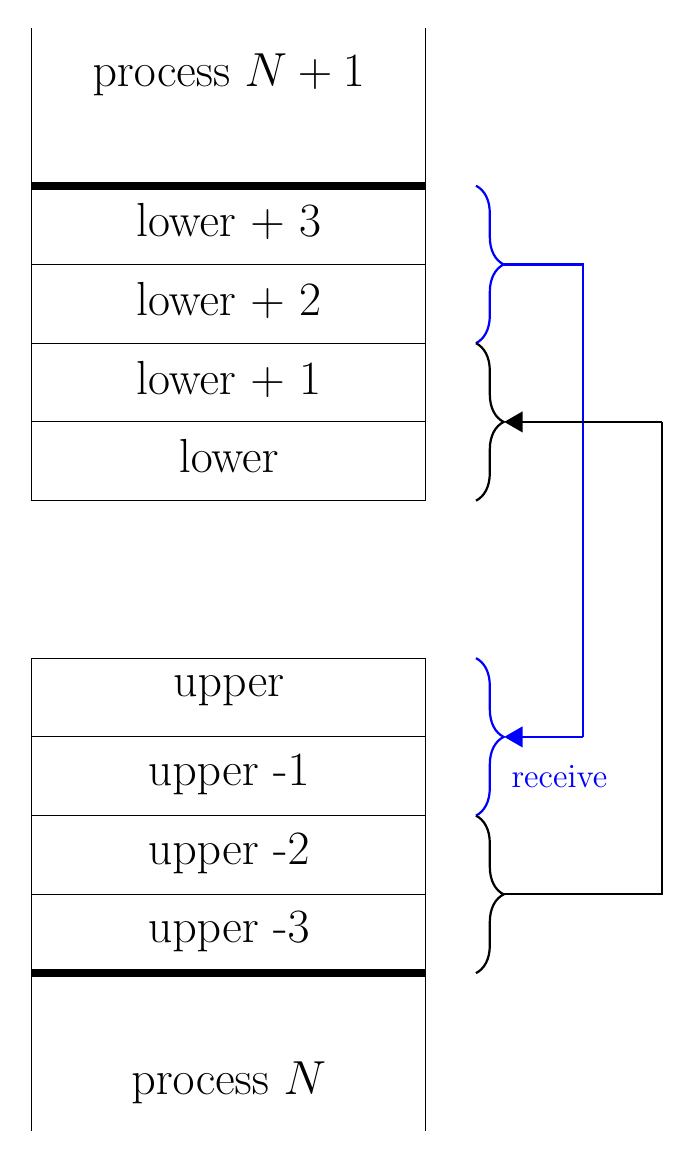
\begin{tikzpicture}[>=triangle 60]
			\draw (0, 2) -- (0, 0) -- (5, 0) -- (5, 2) node [right = -2.5cm, below = 0.2cm] {\LARGE process $N +1$};
			\draw (0, 0) -- (5, 0) -- (5, -1) -- (0, -1) -- (0, 0) node [right = 2.5cm, below = 0.1cm] {\LARGE lower + 3};
			\draw [line width = 3pt] (0, 0) -- (5, 0);
			\draw (0, -1) -- (5, -1) -- (5, -2) -- (0, -2) -- (0, -1) node [right = 2.5cm, below = 0.1cm] {\LARGE lower + 2};
			\draw (0, -2) -- (5, -2) -- (5, -3) -- (0, -3) -- (0, -2) node [right = 2.5cm, below = 0.1cm] {\LARGE lower + 1};
			\draw (0, -3) -- (5, -3) -- (5, -4) -- (0, -4) -- (0, -3) node [right = 2.5cm, below = 0.1cm] {\LARGE lower};
			
			\draw (0, -6) -- (5, -6) -- (5, -7) -- (0, -7) -- (0, -6) node [right = 2.5cm, below = 0.1cm] {\LARGE upper};
			\draw (0, -7) -- (5, -7) -- (5, -8) -- (0, -8) -- (0, -7) node [right = 2.5cm, below = 0.1cm] {\LARGE upper -1};
			\draw (0, -8) -- (5, -8) -- (5, -9) -- (0, -9) -- (0, -8) node [right = 2.5cm, below = 0.1cm] {\LARGE upper -2};
			\draw (0, -9) -- (5, -9) -- (5, -10) -- (0, -10) -- (0, -9) node [right = 2.5cm, below = 0.1cm] {\LARGE upper -3};
			\draw (0, -12) -- (0, -9) -- (5, -9) -- (5, -12) node [right = -2.5cm, below = -1cm] {\LARGE process $N$};
			\draw [line width = 3pt] (0, -10) -- (5, -10);
			\draw [blue,decorate,decoration={brace,amplitude=10pt,mirror,raise=4pt}, thick,yshift=0pt]
(5.5,-2) -- (5.5,0) node [black,xshift=0.8cm] {};
			\draw [decorate,decoration={brace,amplitude=10pt,mirror,raise=4pt}, thick,yshift=0pt]
(5.5,-4) -- (5.5,-2) node [black,xshift=0.8cm] {};
			\draw [blue,decorate,decoration={brace,amplitude=10pt,mirror,raise=4pt},  thick,yshift=0pt]
(5.5,-8) -- (5.5,-6) node [black,xshift=0.8cm] {};
			\draw [decorate,decoration={brace,amplitude=10pt,mirror,raise=4pt}, thick,yshift=0pt]
(5.5,-10) -- (5.5,-8) node [black,xshift=0.8cm] {};
			\draw[blue, thick] (6, -1) -- (7, -1) -- (7, -7);
			\draw [thick] (6, -9) -- (8, -9) -- (8, -3);
    		\draw [blue,arrow, thick] (7, -7) -- (6, -7);
    		\draw [arrow, thick] (8, -3) -- (6, -3);
		
		\node[blue, thick] (rcv) at (6.7,-7.5) {\large receive};
		
		\end{tikzpicture}
		}
		\caption{Second step for odd-numbered processes}
		\label{fig:steptwo}
		\end{minipage}
		\end{center}
\end{figure}


As illustrated in Figure \ref{fig:stepone} and Figure \ref{fig:steptwo}, the thick lines are joined together in the actual simulation output. This behaviour can be achieved by letting the different processes communicate to each other in the following way:\\
First the odd-numbered processes send their values to the above and below processes (Figure \ref{fig:stepone}), while the even-numbered ones receive from below and above, respectively. Then, this procedure is repeated with the even-numbered ones sending and the odd-numbered ones receiving (Figure \ref{fig:steptwo}). Special attention has to be paid to the lower most and the upper most process, because they do only have to send and receive from one border. The main reason to implement the comunication in this way, was to avoid a deadlock.\\
Other components of the code that needed to be adjusted were workspace allocation, time step computation and output formatting.




\subsubsection{Results}
To evaluate the performance of the parallelized code, a \textit{strong} and a \textit{weak scaling} was performed. More precisely, for the strong scaling we ran the code with 1 to 36 cores and a $ny$ of 9000 units. This was repeated ten times to get a mean time per core. Similarly, for the weak scaling we varied the number of cores from 1 to 36, each time incrementing $ny$ by 300 units to keep the grid size per core constant. The results of the respective runtimes are displayed in Figure \ref{fig:runtimes}.

\begin{figure}[htbp]
	\begin{minipage}{0.49\textwidth} 
	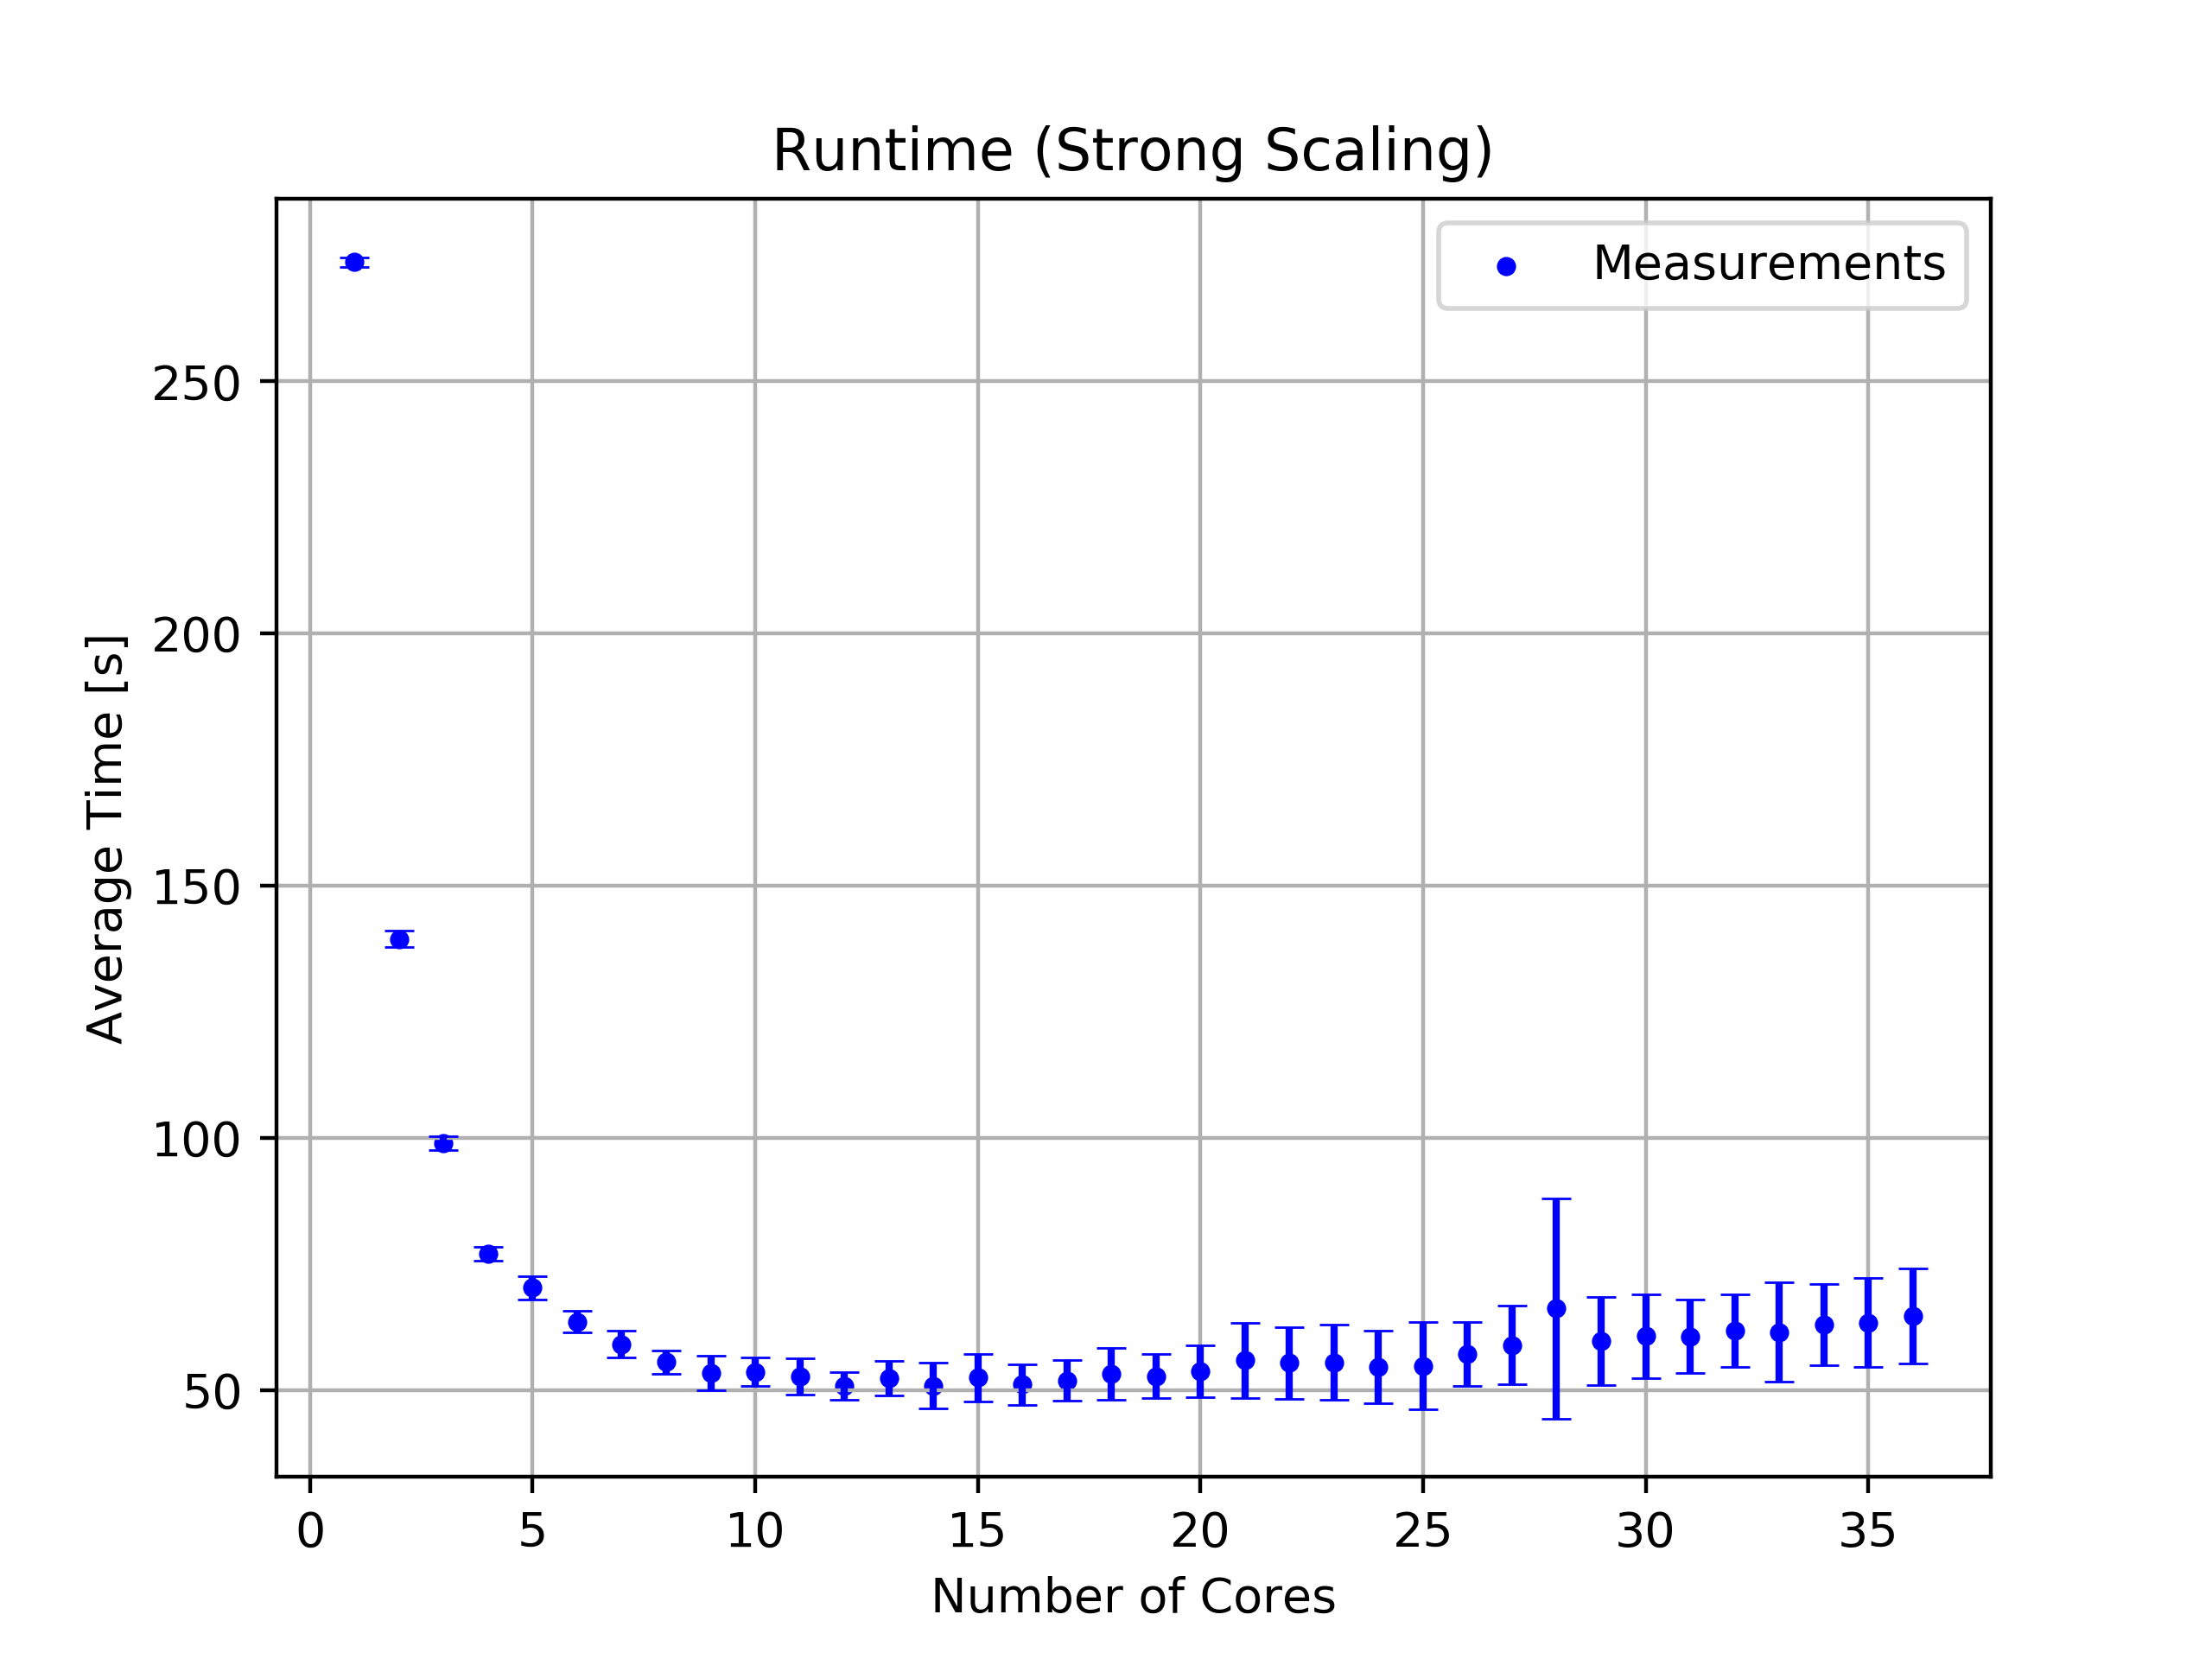
\includegraphics[width=\textwidth]{pictures/avg_strong.png}
	\end{minipage}
	\hfill
	\begin{minipage}{0.49\textwidth}
	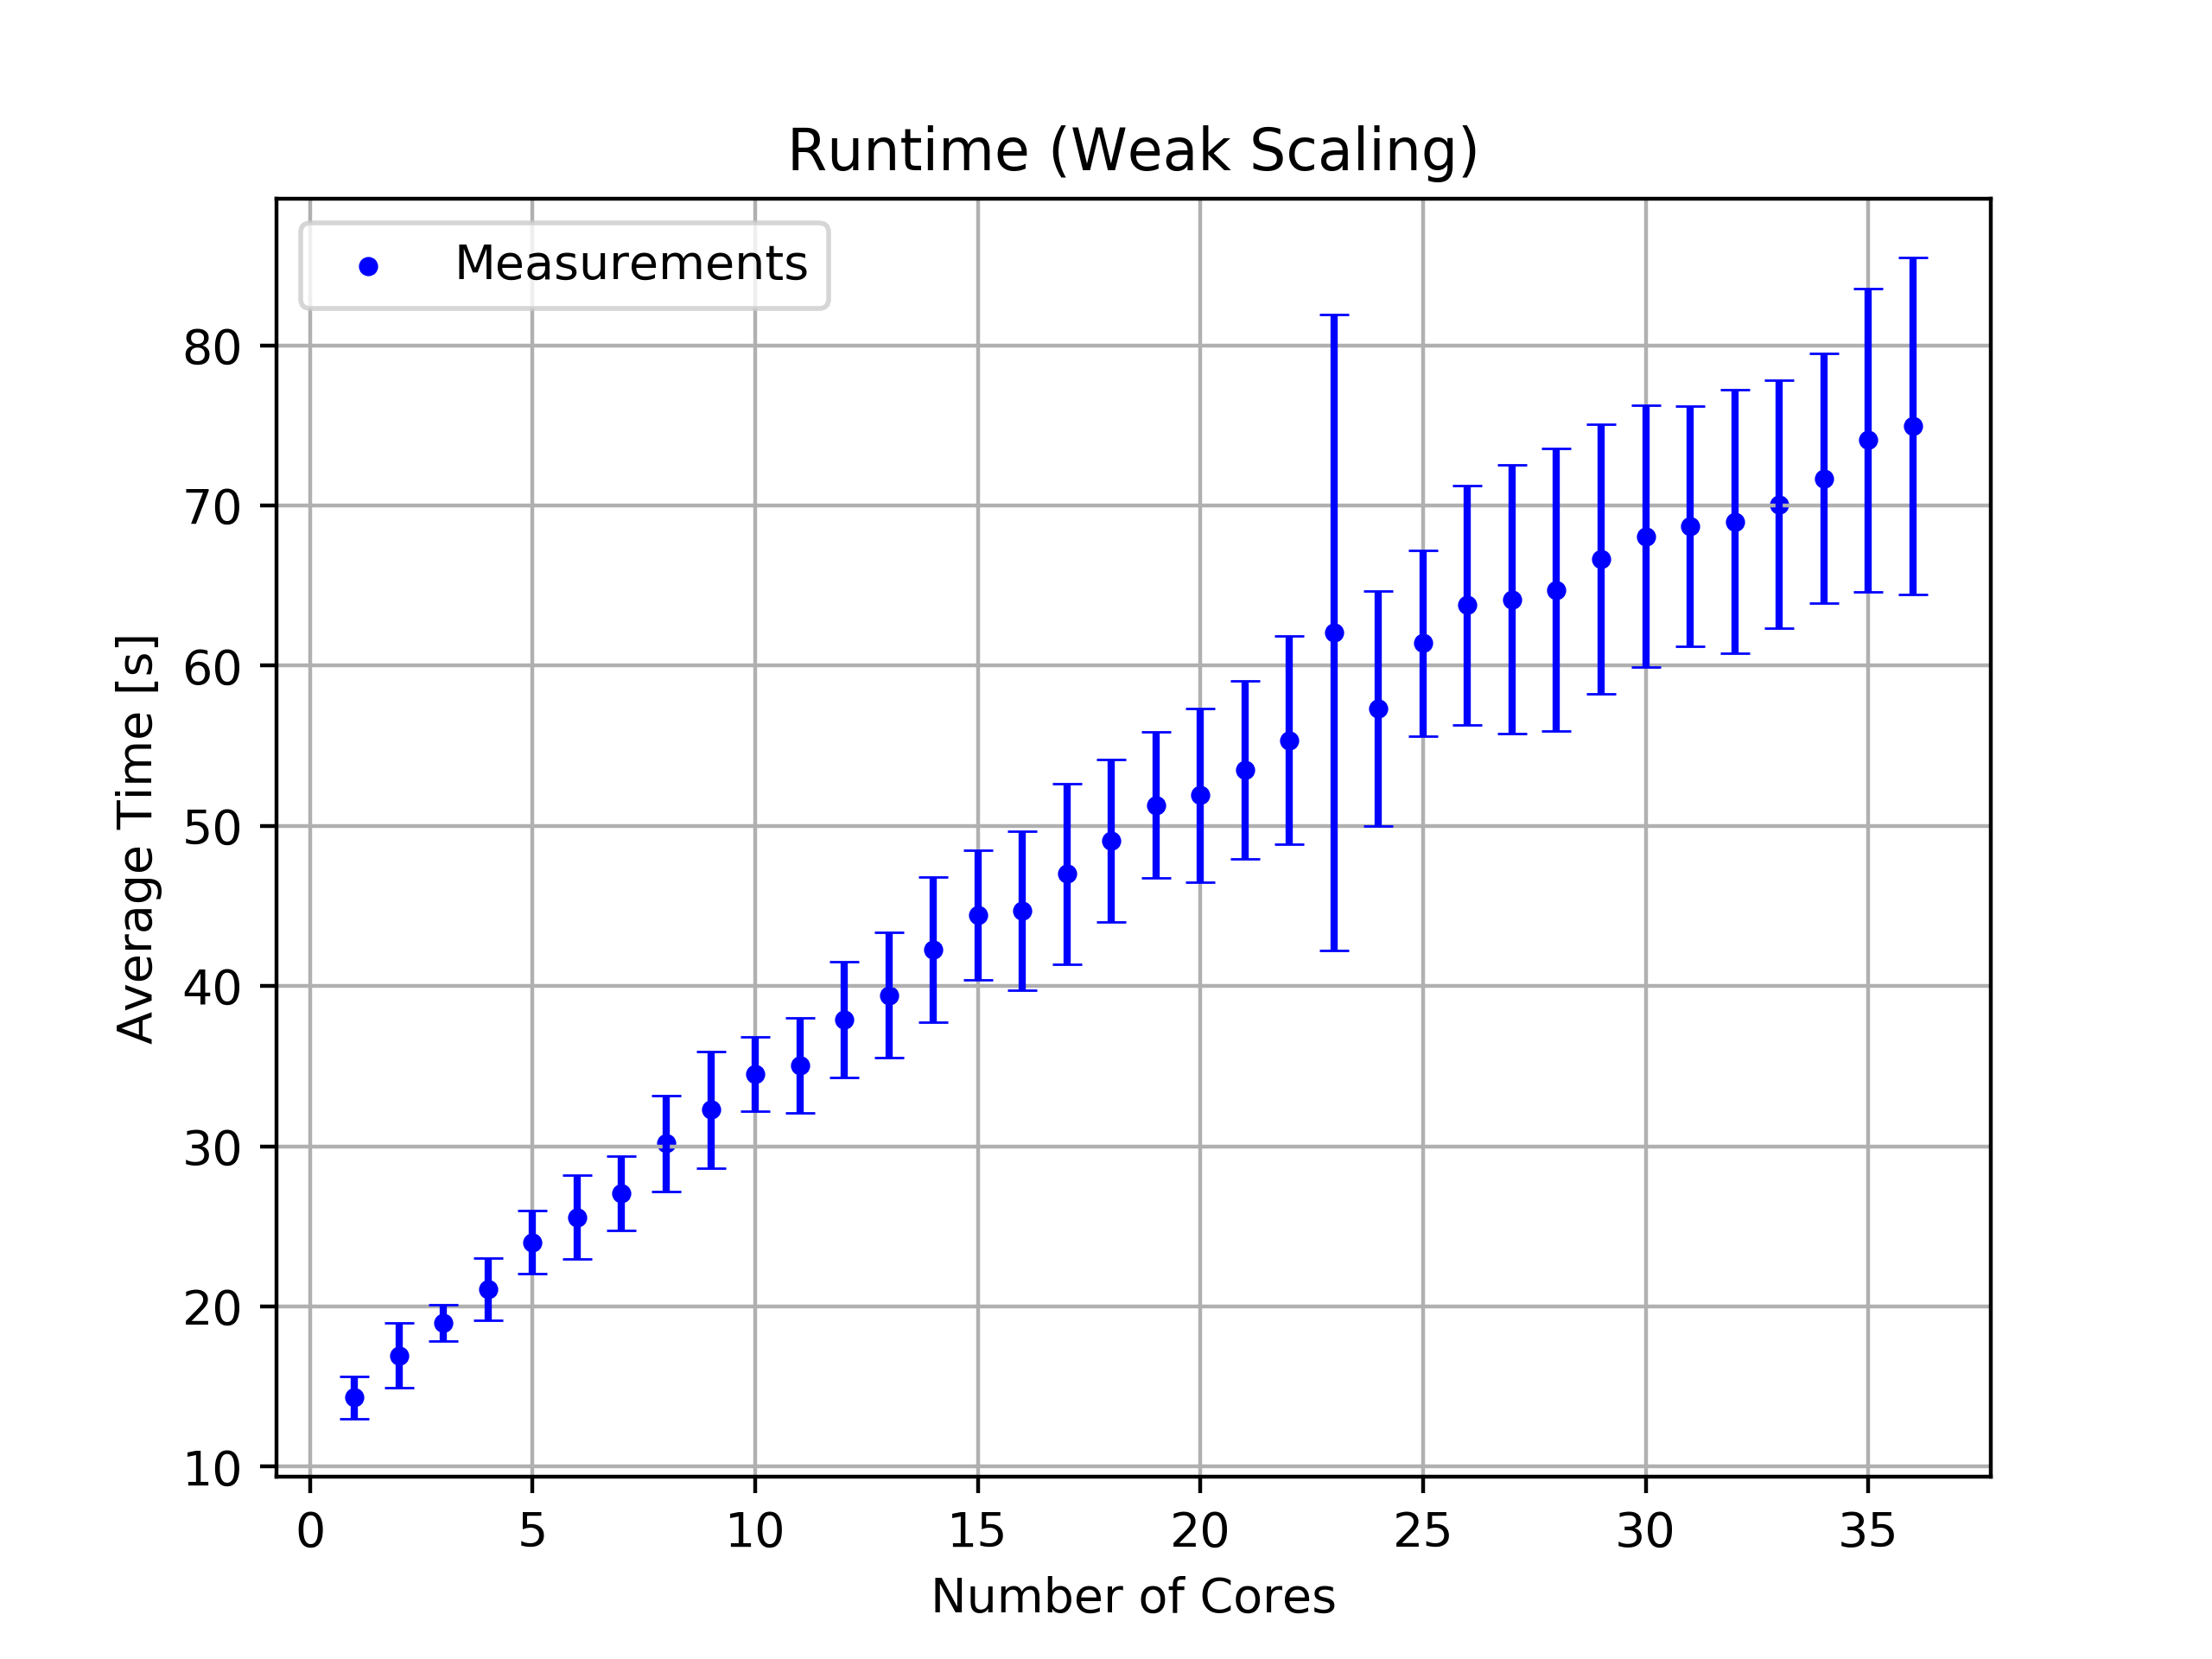
\includegraphics[width=\textwidth]{pictures/avg_weak.png}
	\end{minipage}
	\label{fig:runtimes}
	\caption{Respective runtimes for strong and weak scaling}
	\label{fig:runtimes}
\end{figure}



%
%The simulation was run from 1 to 36 cores 10 times each.
%
%The settings for the strong scaling were the following:\\
%\begin{center}
%\begin{tabular}{c|c|c|c}
% $t_{\text{end}}$ & $nx$ & $ny$ & $\der x$ \\ \hline
% 50.0 & 50 & 9000 & 0.08 \\
%\end{tabular}
%\end{center}
%
%The settings for the weak scaling were the following:\\
%\begin{center}
%\begin{tabular}{c|c|c|c}
% $t_{\text{end}}$ & $nx$ & $ny$ & $\der x$ \\ \hline
% 50.0 & 50 & 300 & 0.08 \\
%\end{tabular}
%\end{center}
%
%Note that the $nx$ remained unchanged during the weak scaling run, but $ny$ increased linearly with the number of processes involved, $ny = ny \cdot $ (number of processes).

To specify the percentage of the code that has actually been parallelized, we analyized the speedup (strong scaling) and the efficiency (weak scaling).\\
In case of the strong scaling, the speedup $s(N)$ is given by
\begin{equation}
	s(N) = \frac{t_\text{s}}{t_\text{p}(N)}=\frac{1}{\alpha + \frac{1-\alpha}{N}},
\end{equation}
where $t_\text{s}$ is the runtime of the serial code (i.e. one core), $t_\text{p}(N)$ is the paralellized code as a function of the number of processes $N$ and $\alpha$ is the non-parallelized fraction of the code. It is displayed in Figure \ref{fig:speedup}.\\

\begin{figure}[h!]
\begin{center}
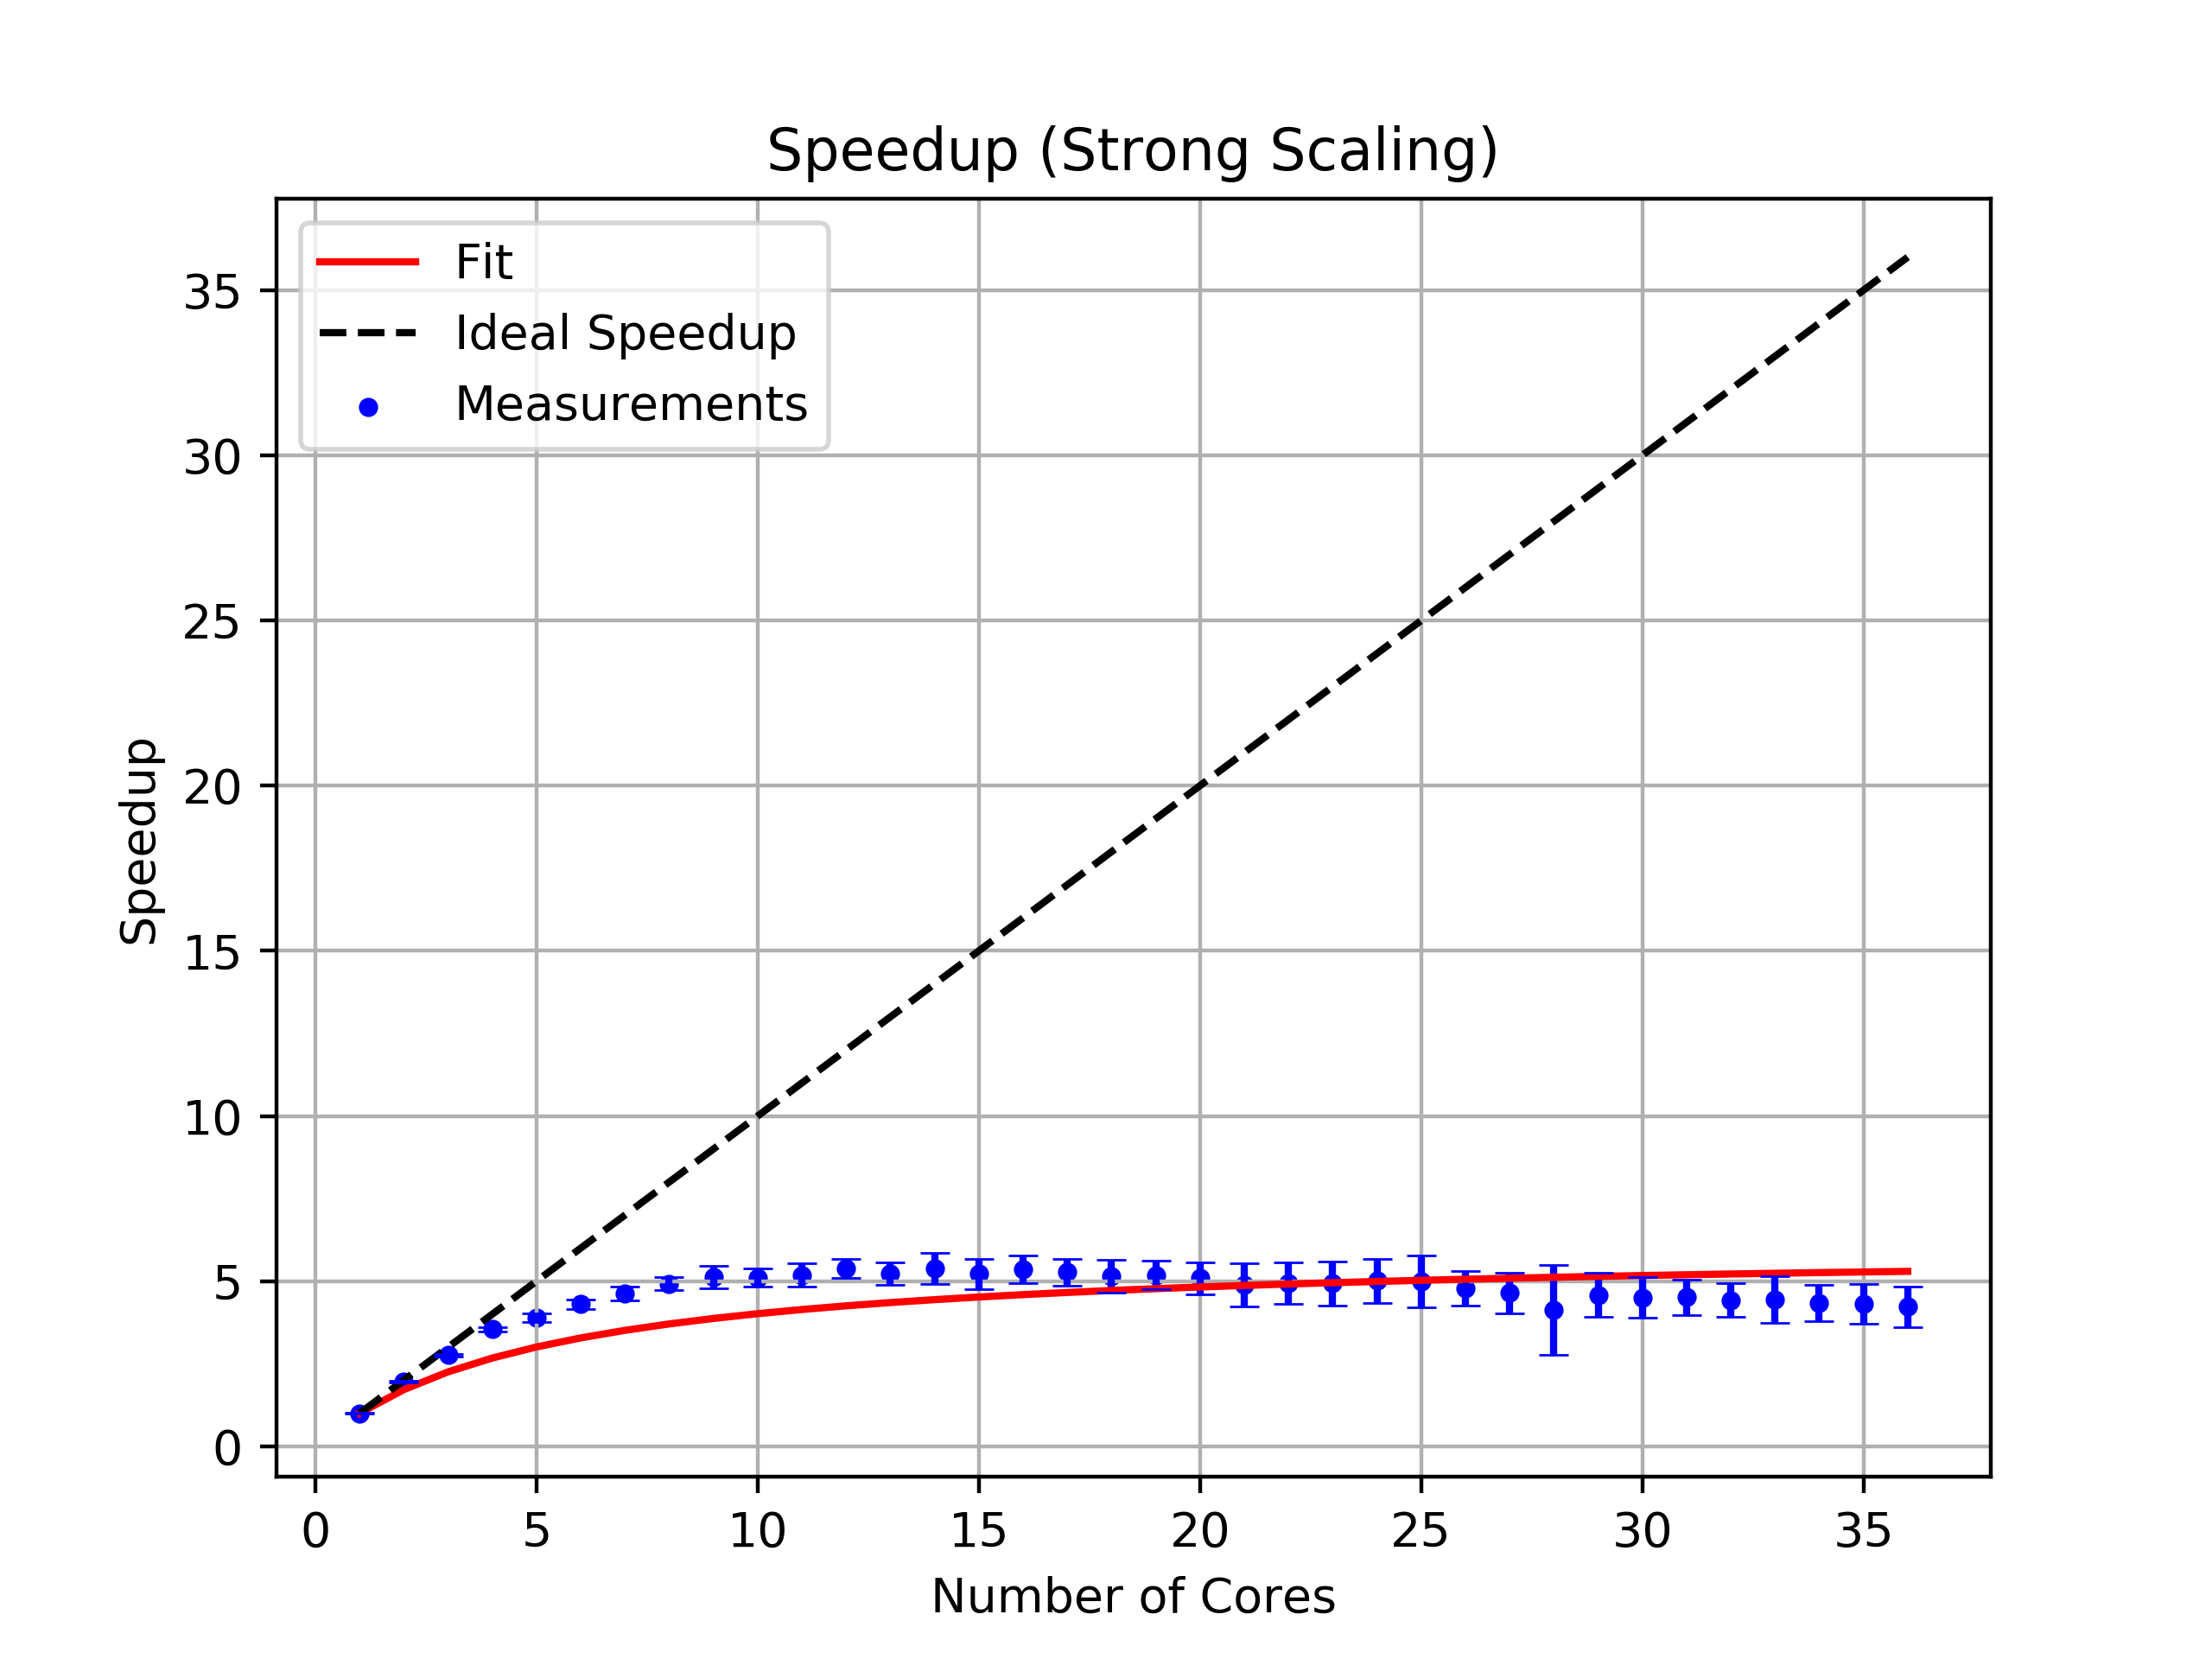
\includegraphics[width=0.8\textwidth]{pictures/speedup_strong.png}
\caption{Speedup for strong scaling.}
\label{fig:speedup}
\end{center}
\end{figure}

The actual value for $\alpha$ can be obtained by fitting the function
\begin{equation}
f(N)=\frac{1}{\alpha + \frac{1-\alpha}{N}}
\end{equation}
to the measurement points. In our case,
\begin{equation} 
\alpha = 0.166 \pm 0.006.
\end{equation}
This indicates that roughly $83.4\%$ of the code is parallelized.

\newpage
In case of the weak scaling, the efficiency $\varepsilon$ is given by
\begin{equation*}
	\varepsilon (N) = \frac{t_\text{s}}{t_\text{p}(N)} = 	\frac{1}{\alpha\cdot N + (1-\alpha)}.
\end{equation*} 
It is illustrated in Figure \ref{fig:efficiency}. Fitting the function to the measurements yields


%The formula for the fit for the weak scaling can be derived quite easily. Again, take $\alpha$ to be the non parallelized fraction of the code. Then, $T_p(N)$, the time needed for the parallel code, is\\
%\begin{equation*}
%T_p(N) = N \cdot \alpha + (1-\alpha)
%\end{equation*} 
%
%So then, 
%\begin{equation*}
%\text{Speedup($N$)} = \frac{T_s(N)}{T_p(N)} = \frac{T_s}{T_p(N)} = \frac{1}{(\alpha)\cdot N + (1-\alpha)}
%\end{equation*} 


\begin{equation}
\alpha = 0.145 \pm 0.002.
\end{equation}
Again, this indicates that around $85.5\%$ of the code is parallelized.

\begin{figure}[h!]
\begin{center}
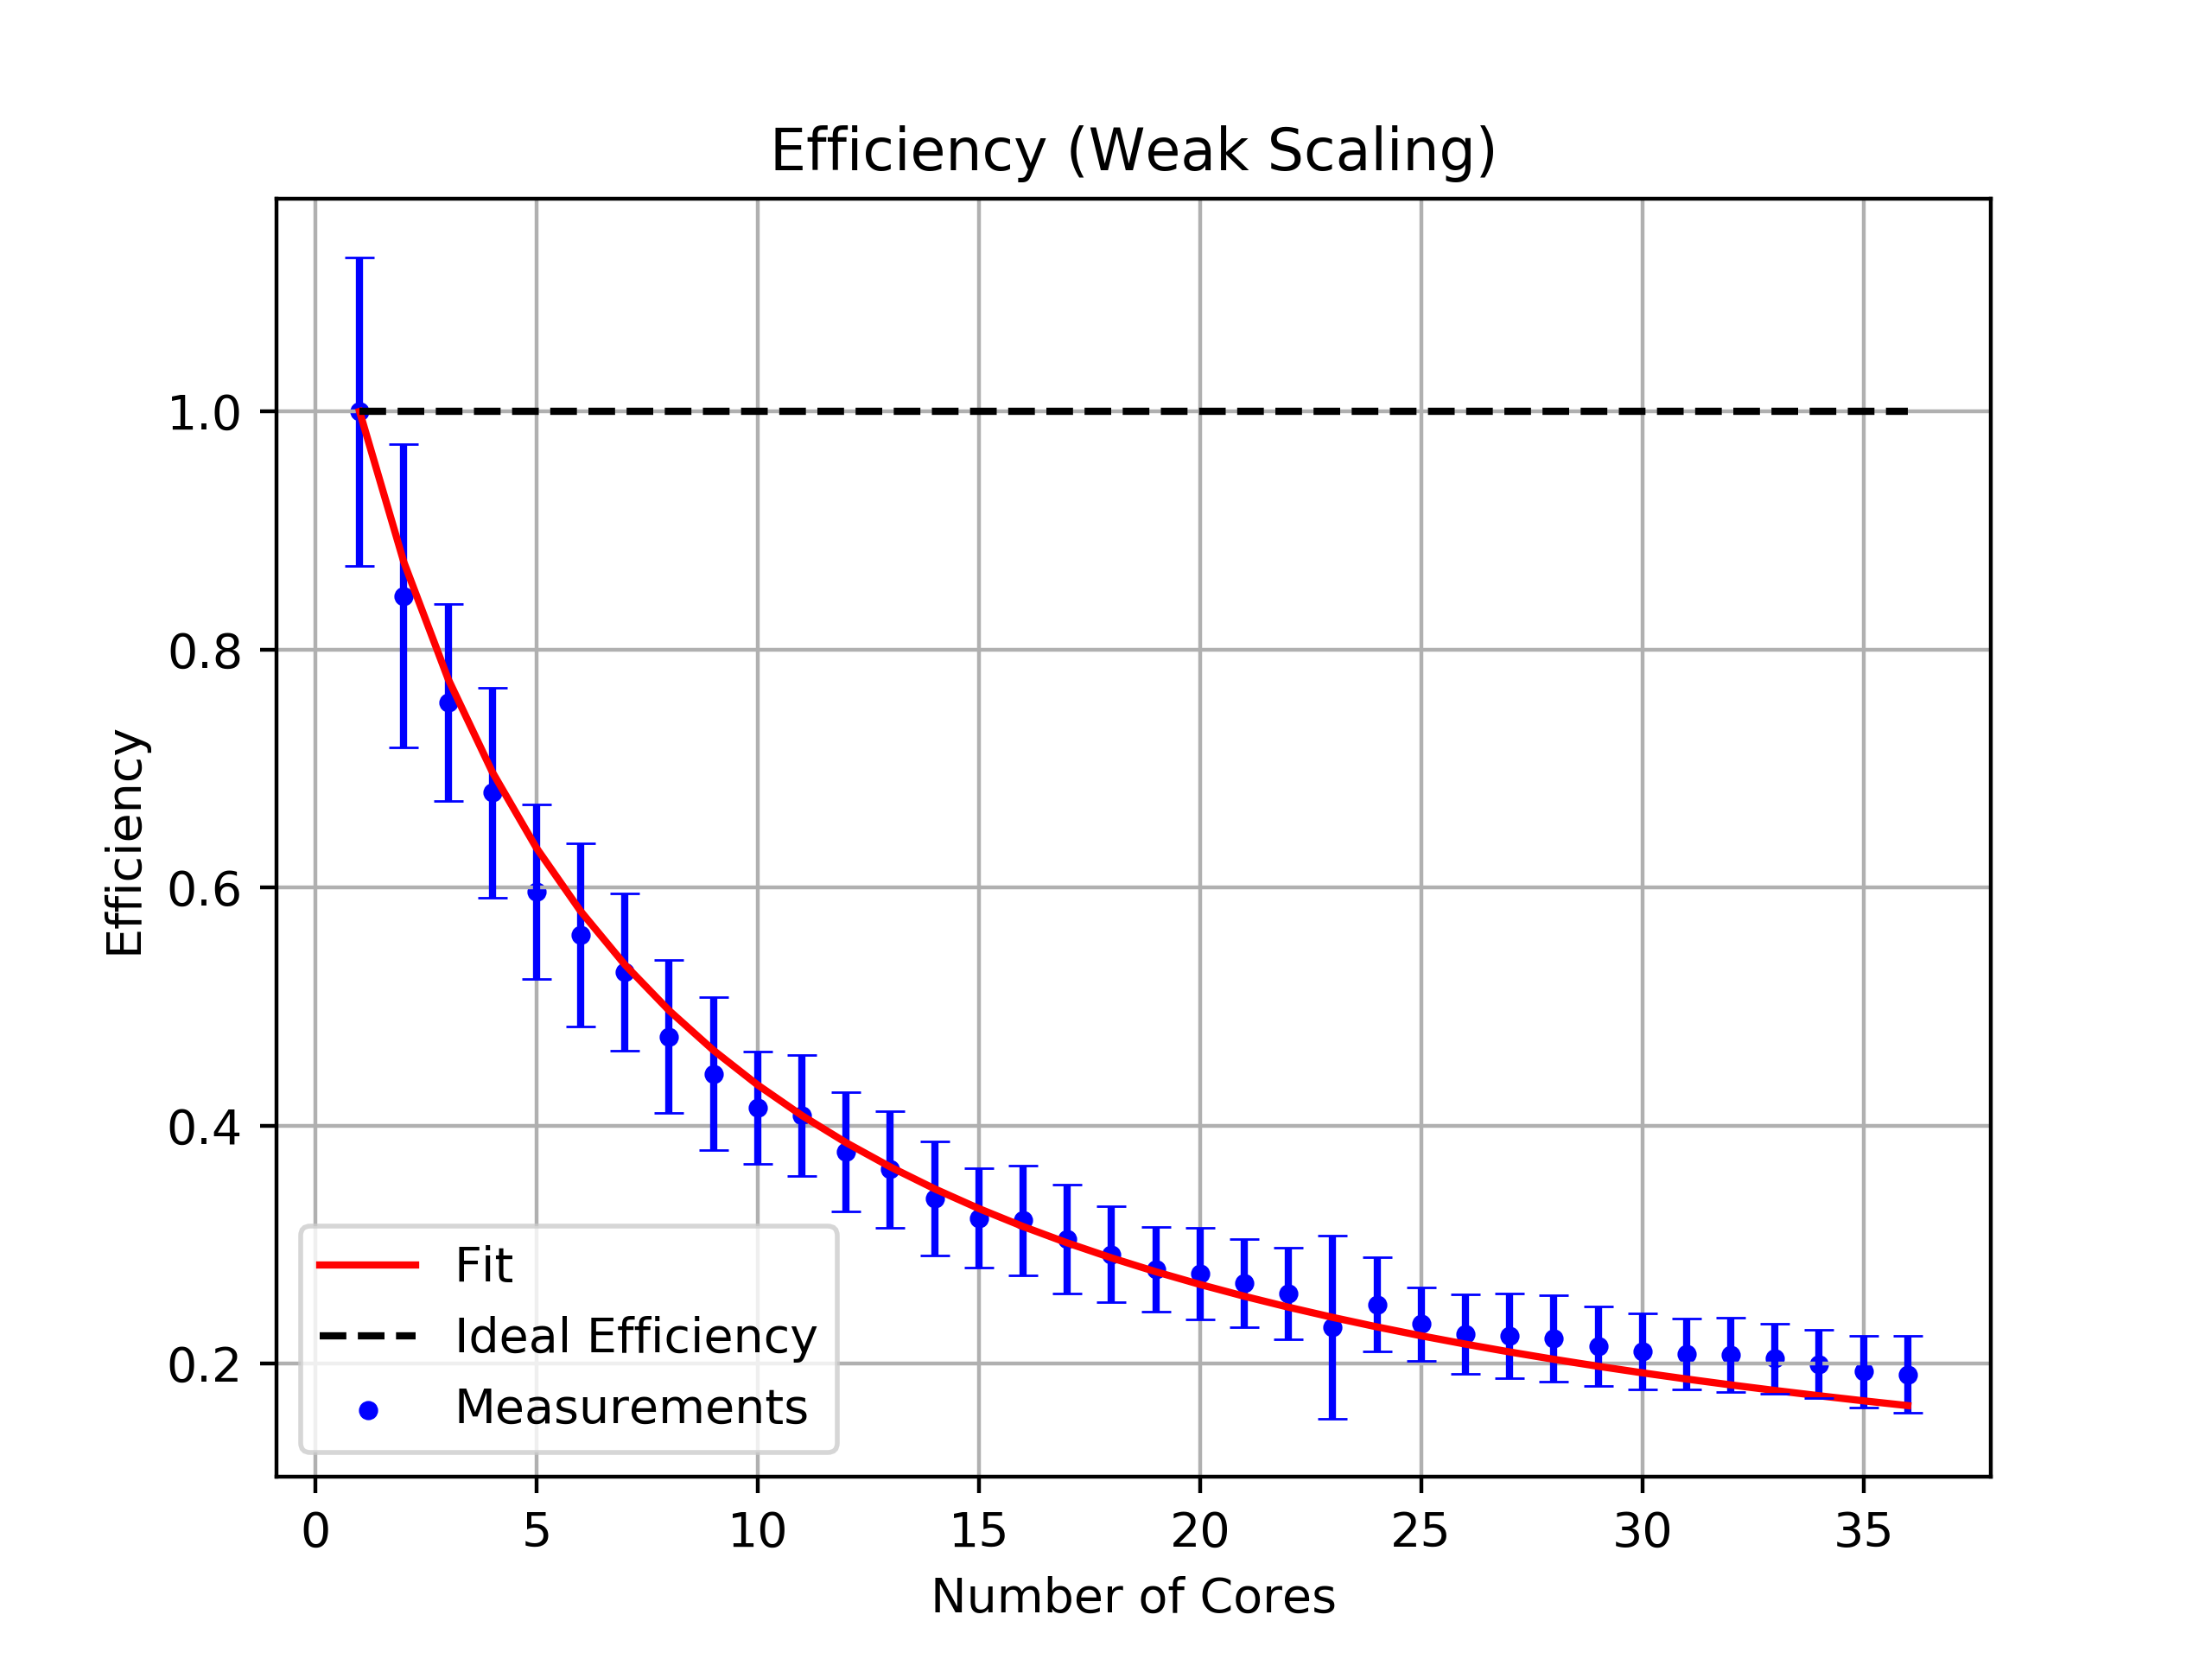
\includegraphics[width=0.8\textwidth]{pictures/speedup_weak.png}
\end{center}
\caption{Efficiency for weak scaling.}
\label{fig:efficiency}
\end{figure}


\newpage
\subsection{Other Techniques}

\subsubsection{OpenMP}

OpenMP stands for \textit{open multiprocessing}. 
The fundamental difference between this and MPI is the parallelization process. MPI communicates between nodes, whereas with OpenMP the parallelization occurs within one node. 

\begin{figure}[h!]
\centering
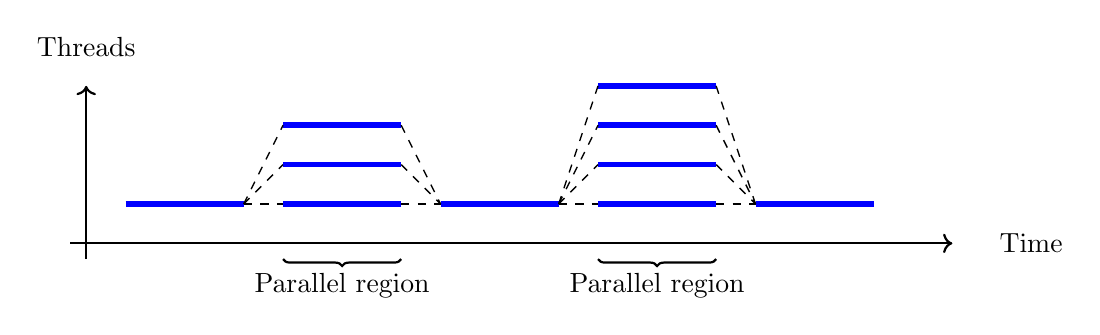
\begin{tikzpicture}
\draw[->, thick] (-0.2,0) -- (11,0);
\draw[->, thick] (0,-0.2) -- (0,2);

\draw[line width=2pt, blue] (0.5,0.5) -- (2,0.5);
\draw[line width=2pt, blue] (2.5,0.5) -- (4,0.5);
\draw[line width=2pt, blue] (2.5,1) -- (4,1);
\draw[line width=2pt, blue] (2.5,1.5) -- (4,1.5);
\draw[line width=2pt, blue] (4.5,0.5) -- (6,0.5);
\draw[line width=2pt, blue] (6.5,0.5) -- (8,0.5);
\draw[line width=2pt, blue] (6.5,1) -- (8,1);
\draw[line width=2pt, blue] (6.5,1.5) -- (8,1.5);
\draw[line width=2pt, blue] (6.5,2) -- (8,2);
\draw[line width=2pt, blue] (8.5,0.5) -- (10,0.5);

\draw[dashed, line width=0.5pt] (2,0.5) -- (2.5,0.5);
\draw[dashed, line width=0.5pt] (2,0.5) -- (2.5,1);
\draw[dashed, line width=0.5pt] (2,0.5) -- (2.5,1.5);
\draw[dashed, line width=0.5pt] (4,0.5) -- (4.5,0.5);
\draw[dashed, line width=0.5pt] (4,1) -- (4.5,0.5);
\draw[dashed, line width=0.5pt] (4,1.5) -- (4.5,0.5);
\draw[dashed, line width=0.5pt] (6,0.5) -- (6.5,0.5);
\draw[dashed, line width=0.5pt] (6,0.5) -- (6.5,1);
\draw[dashed, line width=0.5pt] (6,0.5) -- (6.5,1.5);
\draw[dashed, line width=0.5pt] (6,0.5) -- (6.5,2);
\draw[dashed, line width=0.5pt] (8,0.5) -- (8.5,0.5);
\draw[dashed, line width=0.5pt] (8,1) -- (8.5,0.5);
\draw[dashed, line width=0.5pt] (8,1.5) -- (8.5,0.5);
\draw[dashed, line width=0.5pt] (8,2) -- (8.5,0.5);

\draw [
    thick,
    decoration={
        brace,
        mirror,
        raise=0.5cm
    },
    decorate
] (2.5,0.3) -- (4,0.3) 
node [pos=0.5,anchor=north,yshift=-0.55cm] {Parallel region}; 

\draw [
    thick,
    decoration={
        brace,
        mirror,
        raise=0.5cm
    },
    decorate
] (6.5,0.3) -- (8,0.3) 
node [pos=0.5,anchor=north,yshift=-0.55cm] {Parallel region}; 



\node (T) at (0,2.5) {Threads}; 
\node (P) at (12,0) {Time}; 
\end{tikzpicture}
\caption{Operating principle of OpenMP}
\label{fig:openmp}
\end{figure}


As illustrated in Figure \ref{fig:openmp}, the so-called \textit{master thread} spawns several \textit{slave threads} (in a process called forking) to speed up a designated section of the code. The individual results are then recombined at the end of such a segment (which is called joining). This parallelization process is mostly used to speed up \textit{for loops}.\\
What it may lack in flexibility (it can only run on shared-memory computers), it makes up in ease of implementation and communication speed. 




\subsubsection{MPI - OpenMP Hybrid}

Implementing both of these methods can make use of the distributed memory architecture of a supercomputer, while further speeding up the runtime by occupying multiple threads. This combines the advantages of both MPI and OpenMP.



\newpage
\section{Discussion}


As can be seen in Figure \ref{fig:runtimes}, the standard deviation on some of the runtimes can be quite big. This is mainly due that the whole run (going from 1 to 36 processes) was only performed 10 times. If one of these times is abnormally high, averaging over only 10 values will not suppress this spike well enough. This is what happened in our case. In the tenth iteration, one of the processes took twice the time it would normally to complete its calculation. This may be due to a temporary performance drop at the Piz Daint supercomputer.\\\\
Our choice in implementing MPI relied on communications which were $\textit{blocking}$, meaning that execution of the code is halted until receiving ($\texttt{MPI\_RECV()}$) or sending ($\texttt{MPI\_SEND()}$) is terminated. If one were to a use non-blocking approach, the runtime may be reduced even further, which could increase the parallelized fraction of the code $\alpha$.\\
\textcolor{red}{Although more difficult to implement, having a non-blocking implementation allows communication and computation to overlap, resulting generally in increased performance.}

\vp


\section{Conclusion}

The choice of dividing the work along the vertical axis (bigger in size) turned out to be the more beneficial one. As can be seen in in the strong scaling (Figure \ref{fig:speedup}), increasing the number of cores above a certain value for a fixed grid size gives diminishing returns, as more time is lost with communications. Also, there is a maximum number of processors that can be used to carry out a simulation of fixed size, as each process needs \textcolor{red}{at least 9 rows to be able to function properly.}\\
Another possibility would be to split the grid both horizontally and vertically. This could be beneficial if one were to work on a square problem. 








\end{document}
